\documentclass[a4paper,fleqn,12pt]{article}

\usepackage[utf8]{inputenc}
\usepackage[bulgarian]{babel}
\usepackage{amsmath}
\usepackage{amssymb}
\usepackage{booktabs}
\usepackage{fancyhdr}
\usepackage{amsthm}
\usepackage{graphicx}
\usepackage{pdfpages}
\usepackage{color}

%\pagestyle{fancy}
%\fancyhf{}
%\lhead{\rightmark}
%\rhead{\thepage}
%\cfoot{}
%\renewcommand{\headrulewidth}{0pt}

%\sloppy
%\definecolor{lightgray}{gray}{0.5}
%\setlength{\parindent}{0pt}



\begin{document}
\begin{titlepage}
	\setlength{\parindent}{0pt}
	\large
\centering
Технически университет -  София \par
Факултет по приложна математика и информатика \par
\vspace{2cm}

{\huge Курсова работа \par}

\vspace{2cm}

\vspace{1cm}
{\LARGE\scshape Числено моделиране с обикновенни диференциални уравнения \par}



\vfill

\begin{minipage}[t]{.5\linewidth}
	Студент: \\
	Кристиян Кръчмаров
\end{minipage}%
\begin{minipage}[t]{.5\linewidth}
	\raggedleft
	Преподавател:\\
	доц. д-р. Богдан Гилев
\end{minipage}

\vspace{2cm}
\raggedright

\end{titlepage}
\tableofcontents
\newpage

\section{Задачи}
\subsection{Задача 1}
Да се реши системата по Рунге - Кута: 
	\begin{gather}
		\begin{array}{|l@{}}
		\frac{dy_1}{dx} = y_2 \\
		\frac{dy_2}{dx} = f(x,y_1,y_2)
		\end{array} \qquad \qquad  \text{при} \qquad \qquad 
		\begin{array}{|l@{}}
		y_1(0) = 0\\
		y_2(0) = y_{20}
		\end{array}\\
		\text{където:} \nonumber \\
		f(x,y_1,y_2) = -axy_2 - x^2y_1 \quad a=0.05 \quad y_{20} = -\frac{1}{6} \nonumber
	\end{gather}

\subsection{Задача 2}
Да се сведе до система и да се реши по метода на матричната експонента уравнението при нулеви начални условия
	\begin{equation}
	y''+3y'=xe^{-2x}
	\end{equation}

\subsection{Задача 3}
Да се реши граничната задача по метода на крайните разлики
	\begin{equation}
	x'' + \frac{1}{t} x' + \left( \frac{16}{t^2}\right) x = \sin \left( \frac{1}{t^2}\right) \quad t \in [1;4]; \, x(1) = -0.3 ; \, x(4) = 0.4
	\end{equation}

\subsection{Задача 4}
Да се реши граничната задача по метода на стрелбата
	\begin{equation}
	x'' + \frac{1}{t} x' + \left( \frac{16}{t^2}\right) x = \sin \left( \frac{1}{t^2}\right) \quad t \in [1;4]; \, x(1) = -0.3 ; \, x(4) = 0.4
	\end{equation}

\newpage
\section{Решения}
\subsection{Задача 1}
Mетодът на Рунге-Кута от 4ти ред се използва за числено решение на система 
обикновенни диференциални уравнения от вида.
	\begin{gather*}
		\begin{array}{|l@{}}
		\frac{dy_1}{dx} = g(x,y_1,y_2) \\
		\frac{dy_2}{dx} = f(x,y_1,y_2)
		\end{array}
		\qquad \qquad  \text{при} \qquad \qquad 
		\begin{array}{|l@{}}
		y_1(x_0) = y_{10}\\
		y_2(x_0) = y_{20}
		\end{array} \\
		\text{където:}  \\
		y_1 = y_1(x) ; \, y_2 =y_2(x) 
	\end{gather*}
Методът се базира на апроксимация на следващата стойност на фунцкията, 
като използва няколко променливи за изчисляване на инкрементацията. 
При Метод на Рунге-Кута от 4ти ред се използват следните променливи
	\begin{gather*}
		k_{1,1} = h \cdot f(x_i,y_{1i}, y_{2i})\\
		k_{2,1} = h \cdot f \left(x_i + \frac{h}{2}, y_{1,i} + \frac{k_{1,1}}{2}, y_{2,i} + \frac{k_{1,2}}{2}\right)\\
		k_{3,1} = h \cdot f \left(x_i + \frac{h}{2}, y_{1,i} + \frac{k_{2,1}}{2}, y_{2,i} + \frac{k_{2,2}}{2}\right)\\
		k_{4,1} = h \cdot f \left(x_i + h, y_{1,i} + k_{3,1}, y_{2,i} + k_{3,2}\right)\\
		y_{1,i+1} = y_{1,i} + \frac{1}{6} \left( k_{1,1} +2k_{2,1} + 2k_{3,1} + k_{4,1}\right)h\\
		\\
		k_{1,2} = h \cdot g(x_i,y_{1i}, y_{2i})\\
		k_{2,2} = h \cdot g \left(x_i + \frac{h}{2}, y_{1,i} + \frac{k_{1,1}}{2}, y_{2,i} + \frac{k_{1,2}}{2}\right)\\
		k_{3,2} = h \cdot g \left(x_i + \frac{h}{2}, y_{1,i} + \frac{k_{2,1}}{2}, y_{2,i} + \frac{k_{2,2}}{2}\right)\\
		k_{4,2} = h \cdot g \left(x_i + h, y_{1,i} + k_{3,1}, y_{2,i} + k_{3,2} \right) \\
		y_{2,i+1} = y_{2,i} + \frac{1}{6} \left( k_{1,2} +2k_{2,2} + 2k_{3,2} + k_{4,2}\right)h\\
\end{gather*}
където $y_{1,i}$ и $y_{2,i}$ са предходни приближения, а $y_{1,i+1}$ и $y_{2,i+1}$ са текущи приближения. \\
	\newpage
	\begin{verbatim}
	function firstTask
	% Дефиниране на началните условия
	y0 = [0; -1/6];
	x0 = 0;
	% Дефиниране на стъпката и броя на стъпките
	h = 0.1;
	n = 150;
	% Използване на RK4 функцията
	[x, y] = RK4(@system, x0, y0, h, n);
	figure(1),plot(x,y(1,:),x,y(2,:));
	title('Решение на системата по Рунге-Кута');
	legend('y1', 'y2', 'Location', 'southwest', 'Orientation', 'vertical');
	xlabel('x');
	ylabel('y');
	end
	
	function [x, y] = RK4(f, x0, y0, h, n)
	% f - функция, която връща дясната част на системата
	% x0 - начална точка за решението
	% y0 - началните условия
	% h - стъпка на метода
	% n - брой стъпки
	
	x = x0 + (0:n-1)*h;  % Изчисляваме x стойностите
	y = zeros(length(y0), n);  % Създаваме матрица за y
	y(:,1) = y0;  % Запазваме началните условия в първата колона на y
	for i = 1:n-1
	    k1 = f(x(i), y(:,i));
	    k2 = f(x(i)+0.5*h, y(:,i)+0.5*h*k1);
	    k3 = f(x(i)+0.5*h, y(:,i)+0.5*h*k2);
	    k4 = f(x(i)+h, y(:,i)+h*k3);
	    y(:,i+1) = y(:,i) + h*(k1+2*k2+2*k3+k4)/6;  % Изчисляваме y_i+1
	end
	end
	
	function dydx = system(x, y)
	a = 0.05;
	dydx = [y(2); -a*y(2) - x^2*y(1)];
	end
	\end{verbatim}

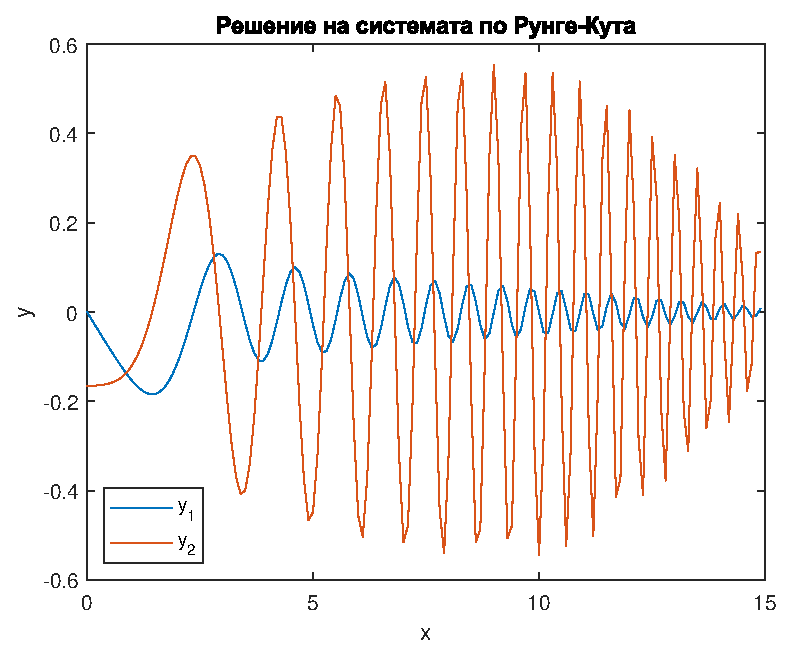
\includegraphics{firstTask_01.eps}

\newpage
\subsection{Задача 2}
Методът на матричната експонента се използва за числено решение на система обикновенни диференциални уравнения от вида 
	\begin{gather*}
		\frac{dy}{dx} = Ay + Bx
		\qquad \qquad  \text{при} \qquad \qquad 
      		y(x_0)=y_0 \\
	\end{gather*}
Матричната експонента се дефинира като безкраен матричен ред
\begin{equation*}
	e^{Ax} = E + \sum_{n=1} ^{\infty} \frac{A^n}{n!}
\end{equation*}
където $E$ е единичната матрица, а $A^n$ е произведението на А, n пъти.\\
В задачата уравнението се свежда до система с въвеждането на 
	\begin{gather*}
		\begin{array}{|l@{}}
			y_1=y\\
			y_2=y'
		\end{array} \implies 
		\begin{pmatrix} y_1 \\ y_2 \end{pmatrix}' = 
		\begin{pmatrix} 0 & 1 \\ 0 & -3 \end{pmatrix} 
		\begin{pmatrix} y_1 \\ y_2 \end{pmatrix} + 
		\begin{pmatrix} 0 \\ xe^{-2x} \end{pmatrix} \iff Y'=AY+B\\ 
		Y'=\begin{pmatrix} y1 \\ y2 \end{pmatrix}' \qquad 
		A=\begin{pmatrix} 0 & 1 \\ 0 & -3 \end{pmatrix} \qquad 
		B=\begin{pmatrix} 0 \\ xe^{-2x} \end{pmatrix} \qquad
		Y=\begin{pmatrix} y1 \\ y2 \end{pmatrix}
	\end{gather*}
Решението на уравнението се дава във вида
\begin{equation*}
	y(x)=e^{A(x-x_0)} y(x_0) + e^{Ax} \int_{x0} ^{x} e^{-As} B(s) \ ds
\end{equation*}
Но, тъй като по условие имаме нулеви начални условия $(y(x_0)=0)$, следва че 
\begin{equation*}
	y(x)=e^{Ax} \int_{x0} ^{x} e^{-As} B(s) \ ds
\end{equation*}
\newpage
\begin{verbatim}
function secondTask
A = [0, 1; -3, 0]; % матрица на коефициенти
B = @(x)[0; myFunction(x)]; % свободни коефициенти
expA = expm(A); % матрична експонента

% начални условия
y0 = [0; 0];
% създаване на масив от времеви точки
t = linspace(0, 10, 200);
% създаване на масив за съхранение на резултатите
y = zeros(length(y0), length(t));

for i = 1:length(t)
    integrand = @(s) expm(A*(t(i)-s)) * B(s);
    y(:,i) = expA * y0 + integral(integrand, 0, t(i), 'ArrayValued', true);
end

figure(2),plot(t, y(1,:),t,y(2,:));
title('Графика на y по метода на матричната експонента');
xlabel('x');
ylabel('y');
legend('y1', 'y2', 'Location', 'northwest', 'Orientation', 'vertical');

end

function f = myFunction(x)
f = x*exp(-2*x);
end
\end{verbatim}

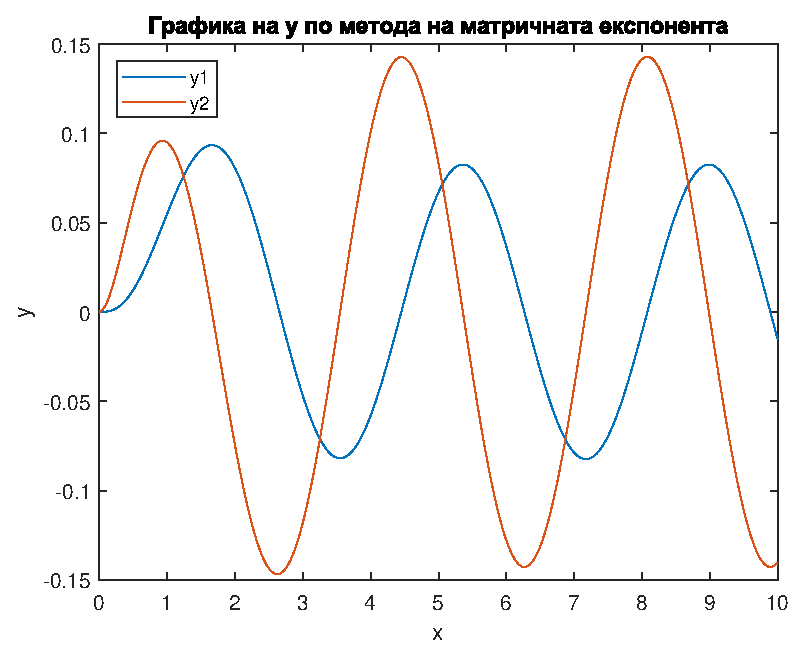
\includegraphics{secondTask_01.eps}

\newpage
\subsection{Задача 3}
Метода на крайните разлики се използва за решаване на обикновенни диференциални уравнения от вида 
\begin{equation*}
	x''(t)=f(t,x,x') \qquad t \in [a;b] \qquad x(a) = \alpha \qquad x(b) = \beta
\end{equation*}
Метода се състои в

\newpage
\begin{verbatim}
function thirdTask
% Задаване на параметри
a = 1; b = 4; % граници на интервала
alpha = -0.3;  beta = 0.4; %x(a)=alpha; x(b)=beta
n = 150; % брой точки на дискретизация
h = (b-a)/(n+1); % стъпка на дискретизация

% Дефиниране на матрицата на коефициентите и вектора на дясната страна
A = zeros(n,n);
f = zeros(n,1);
for i = 1:n
    ti = a + i*h;
    A(i,i) = -2/h^2 + 16/ti^2;
    f(i) = h^2*sin(1/ti^2);
    if i ~= 1
        A(i,i-1) = 1/h^2 - 1/(2*h*ti);
    end
    if i ~= n
        A(i,i+1) = 1/h^2 + 1/(2*h*ti);
    end
end

% Прилагане на граничните условия
A(1,:) = 0; A(1,1) = 1;
f(1) = alpha;
A(n,:) = 0; A(n,n) = 1;
f(n) = beta;

% Решаване на системата
x = A\f;

% Визуализация на решението
t = linspace(a,b,n+2);
xx=[alpha;x;beta];
figure(3),plot(t,xx);
xlabel('t');
ylabel('x(t)');
title('Решение по метода на крайните приближения');
end
\end{verbatim}

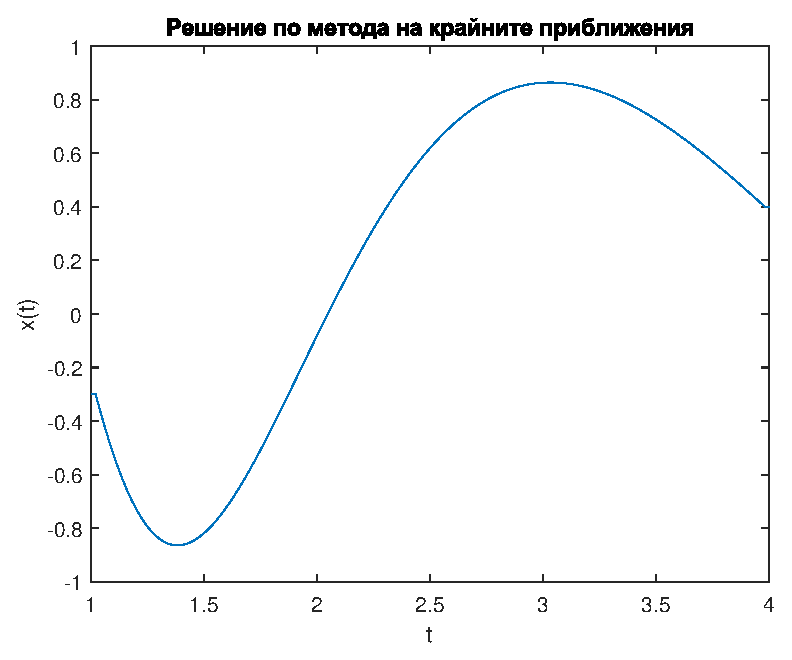
\includegraphics{thirdTask_01.eps}

\newpage
\subsection{Задача 4}
Метода на стрелбата се използва за решаване на обикновенни диференциални уравнения от вида
\begin{equation*}
	x''(t)=f(t,x,x') \qquad t \in [a;b] \qquad x(a) = \alpha \qquad x(b) = \beta
\end{equation*}
\newpage
\begin{verbatim}
function fourthTask
t0=0;
t0=fsolve(@function1,t0);
x0=[-0.3,t0];
[t,x]=ode45(@function2,[1,4],x0);
figure(4),plot(t,x(:,1),t,x(:,2),'r')
xlabel('t');
ylabel('x(t)');
legend('x(t)', "x'(t)", 'Location', 'northeast');
title('Решение по метода на стрелбата');
end

function f=function1(x)
x0=[-0.3,x];
[t,x]=ode45(@function2,[1,4],x0);
n=length(t);
f=x(n,1)-0.4;
end

function dy=function2(t,x)
dy(1,1)=x(2);
dy(2,1)=sin(1/t^2)-(16/t^2)-(x(1)/t);
end
\end{verbatim}
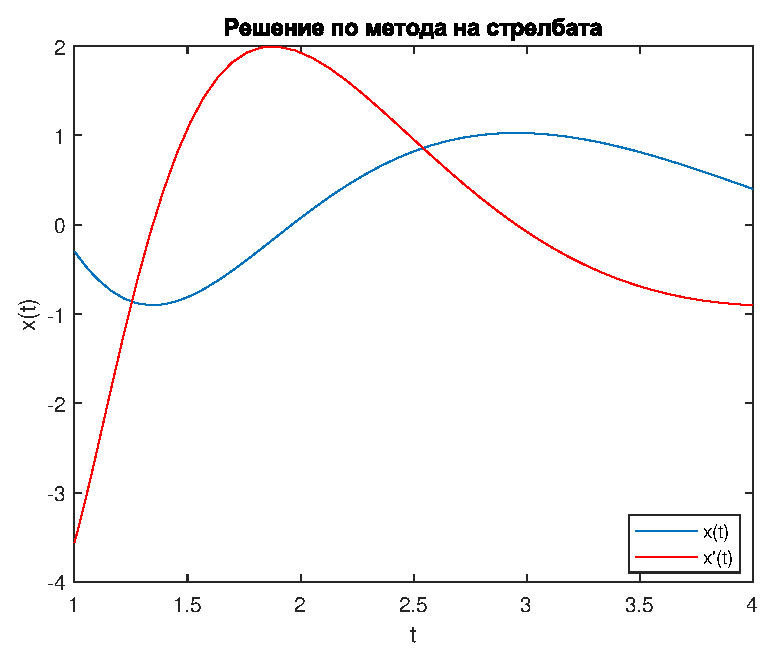
\includegraphics {fourthTask_01.eps}









































































\end{document}